\documentclass[11pt,a4paper]{article}
\usepackage[margin=1in]{geometry}
\usepackage{amsmath,amssymb}
\usepackage{graphicx}
\usepackage{booktabs}
\usepackage{hyperref}
\usepackage{caption}

\hypersetup{colorlinks=true, linkcolor=blue, urlcolor=blue, citecolor=blue}

\title{\textbf{Columnar Reconstruction and Maximum-Likelihood Fitting of $\mu + \tau_h$ Final States in 2016 CMS Open Data at $\sqrt{s} = 13\text{ TeV}$}}
\author{Md Fahad Islam Athoy\\Department of Computer Science \& Engineering, North South University, Dhaka, Bangladesh\\\texttt{fahad.athoy@northsouth.edu} $\cdot$ \href{https://github.com/FahadAthoy01/cms-nanoaod-ditau-analysis}{github.com/FahadAthoy01/cms-nanoaod-ditau-analysis}}
\date{November 2026}

\begin{document}
\maketitle

\begin{abstract}
This technical note presents an end-to-end, reproducible columnar data analysis of opposite-sign muon and hadronically decaying tau ($\mu^\pm\tau_h^\mp$) final states using proton-proton collision data recorded by the CMS experiment in 2016 at $\sqrt{s} = 13\text{ TeV}$ (Run2016H NanoAODv9). Data files are streamed remotely from the CERN EOS public storage system via the \texttt{XRootD} protocol and processed using declarative \texttt{ROOT RDataFrame} pipelines combined with compiled C++17 kinematic kernels. Dominant Standard Model backgrounds from $t\bar{t}$ and $W+\text{jets}$ production are suppressed via a $b$-tagged jet veto and a muon-missing transverse momentum transverse mass cut ($m_T < 40\text{ GeV}$), while quantum chromodynamics (QCD) multijet contributions are estimated directly from data using a same-sign ($\mu^\pm\tau_h^\pm$) control region. A maximum-likelihood fit performed with \texttt{RooFit} extracts a resonance peak at $91.1 \pm 0.7\text{ GeV}$ with resolution $\sigma = 2.9 \pm 0.6\text{ GeV}$ and a signal yield of $N_{\text{sig}} = 22.7 \pm 5.1$ events.
\end{abstract}

\section{Introduction and Physics Motivation}
The reconstruction of di-tau ($\tau^+\tau^-$) final states at the Large Hadron Collider (LHC) forms a cornerstone of electroweak precision measurements ($Z/\gamma^* \to \tau^+\tau^-$) and Yukawa coupling studies of the Higgs boson ($H \to \tau^+\tau^-$). Because the $\tau$ lepton has a proper lifetime of approximately $290\text{ fs}$, it decays inside the beam pipe before reaching active detector layers. In the semi-leptonic $\mu + \tau_h$ channel, one $\tau$ lepton decays leptonically into a muon and two neutrinos ($\tau \to \mu\nu_\mu\nu_\tau$, branching fraction $\approx 17.4\%$), while the second decays hadronically into charged and neutral mesons accompanied by a tau neutrino ($\tau_h + \nu_\tau$, branching fraction $\approx 64.8\%$).

Several Standard Model processes mimic the $\mu + \tau_h$ signature in the CMS detector:
\begin{itemize}
    \item \textbf{Drell-Yan ($Z/\gamma^* \to \tau^+\tau^-$ and $Z/\gamma^* \to \ell^+\ell^-$):} Genuine $Z \to \tau^+\tau^-$ decays yield a shifted visible invariant mass distribution ($60\text{--}85\text{ GeV}$) due to unmeasured neutrino momentum. Conversely, $Z \to \mu^+\mu^-$ events in which one lepton is misidentified as a hadronic $\tau_h$ candidate produce a narrow resonance peak centered near the on-shell $Z$ boson mass ($m_Z = 91.19\text{ GeV}$).
    \item \textbf{$W+\text{jets}$ Production:} A real muon originating from $W \to \mu\nu_\mu$ paired with a quark or gluon jet misidentified as a $\tau_h$ candidate contributes substantially at high transverse mass.
    \item \textbf{Top-Quark Pair Production ($t\bar{t}$):} Decays via $t \to bW$ produce isolated leptons accompanied by bottom-quark jets ($b$-jets).
    \item \textbf{QCD Multijet Production:} High-cross-section multijet events produce non-prompt muons and jet-to-$\tau_h$ fakes at equal rates in opposite-sign (OS) and same-sign (SS) charge configurations.
\end{itemize}

\section{Dataset and Columnar Software Architecture}
The analysis processes $100,000$ collision events from the CMS \texttt{Run2016H SingleMuon} primary dataset in \texttt{NanoAODv9} format (CERN Open Data Portal DOI: \texttt{10.7483/OPENDATA.CMS.A342.9982}). Rather than staging multi-gigabyte files to local storage, the workflow streams event branches on demand over the network from \texttt{root://eospublic.cern.ch/} using \texttt{XRootD} and CERN \texttt{ROOT} v6.40.

To avoid Python event-loop overhead, kinematic computations are implemented as C++17 functions compiled just-in-time via \texttt{ROOT::gInterpreter::Declare} and executed inside the declarative \texttt{ROOT::RDataFrame} graph. In particular, the transverse mass between the selected muon and the missing transverse momentum ($p_T^{\text{miss}}$, branch \texttt{MET\_pt}) is computed as:
\begin{equation}
    m_T(\mu, p_T^{\text{miss}}) = \sqrt{2 p_T^\mu p_T^{\text{miss}} \left(1 - \cos\Delta\phi(\mu, \vec{p}_T^{\text{miss}})\right)},
\end{equation}
and the angular separation in pseudorapidity-azimuth space is defined by $\Delta R = \sqrt{(\Delta\eta)^2 + (\Delta\phi)^2}$.

\section{Event Selection and Background Suppression}
Table~\ref{tab:cuts} summarizes the kinematic and topological selection criteria applied in the \texttt{RDataFrame} pipeline (\texttt{configs/workflow.yaml}).

\begin{table}[h!]
\centering
\caption{Summary of object reconstruction and event selection criteria for the $\mu + \tau_h$ channel.}
\label{tab:cuts}
\begin{tabular}{ll}
\toprule
\textbf{Selection Stage} & \textbf{Kinematic / Identification Requirement} \\
\midrule
Muon Candidate ($\mu$) & $p_T > 25.0\text{ GeV}$, $|\eta| < 2.1$, \texttt{Muon\_tightId == true}, $I_{\text{rel}}^{\text{PF}} < 0.15$ \\
Hadronic Tau Candidate ($\tau_h$) & $p_T > 20.0\text{ GeV}$, $|\eta| < 2.3$ (highest-$p_T$ passing candidate) \\
Lepton-Tau Separation & $\Delta R(\mu, \tau_h) > 0.5$ \\
$t\bar{t}$ Background Veto & Zero jets with $p_T > 20.0\text{ GeV}$, $|\eta| < 2.4$, and \texttt{Jet\_btagCSVV2} $> 0.8484$ \\
$W+\text{jets}$ Suppression & $m_T(\mu, p_T^{\text{miss}}) < 40.0\text{ GeV}$ \\
Signal vs.\ Control Partition & Opposite-Sign ($q_\mu \cdot q_{\tau_h} < 0$) vs.\ Same-Sign ($q_\mu \cdot q_{\tau_h} > 0$) \\
\bottomrule
\end{tabular}
\end{table}

Figure~\ref{fig:recon} illustrates the resulting physical distributions. In the right panel, the $m_T(\mu, p_T^{\text{miss}})$ spectrum exhibits a clear Jacobian peak between $50\text{ GeV}$ and $85\text{ GeV}$ arising from on-shell $W \to \mu\nu$ decays; applying the $m_T < 40\text{ GeV}$ threshold removes this background component. In the left panel, the Same-Sign (SS) QCD estimate remains flat at $\le 2$ events per $5\text{ GeV}$ bin, whereas the Opposite-Sign (OS) data displays a pronounced resonant excess.

\begin{figure}[h!]
    \centering
    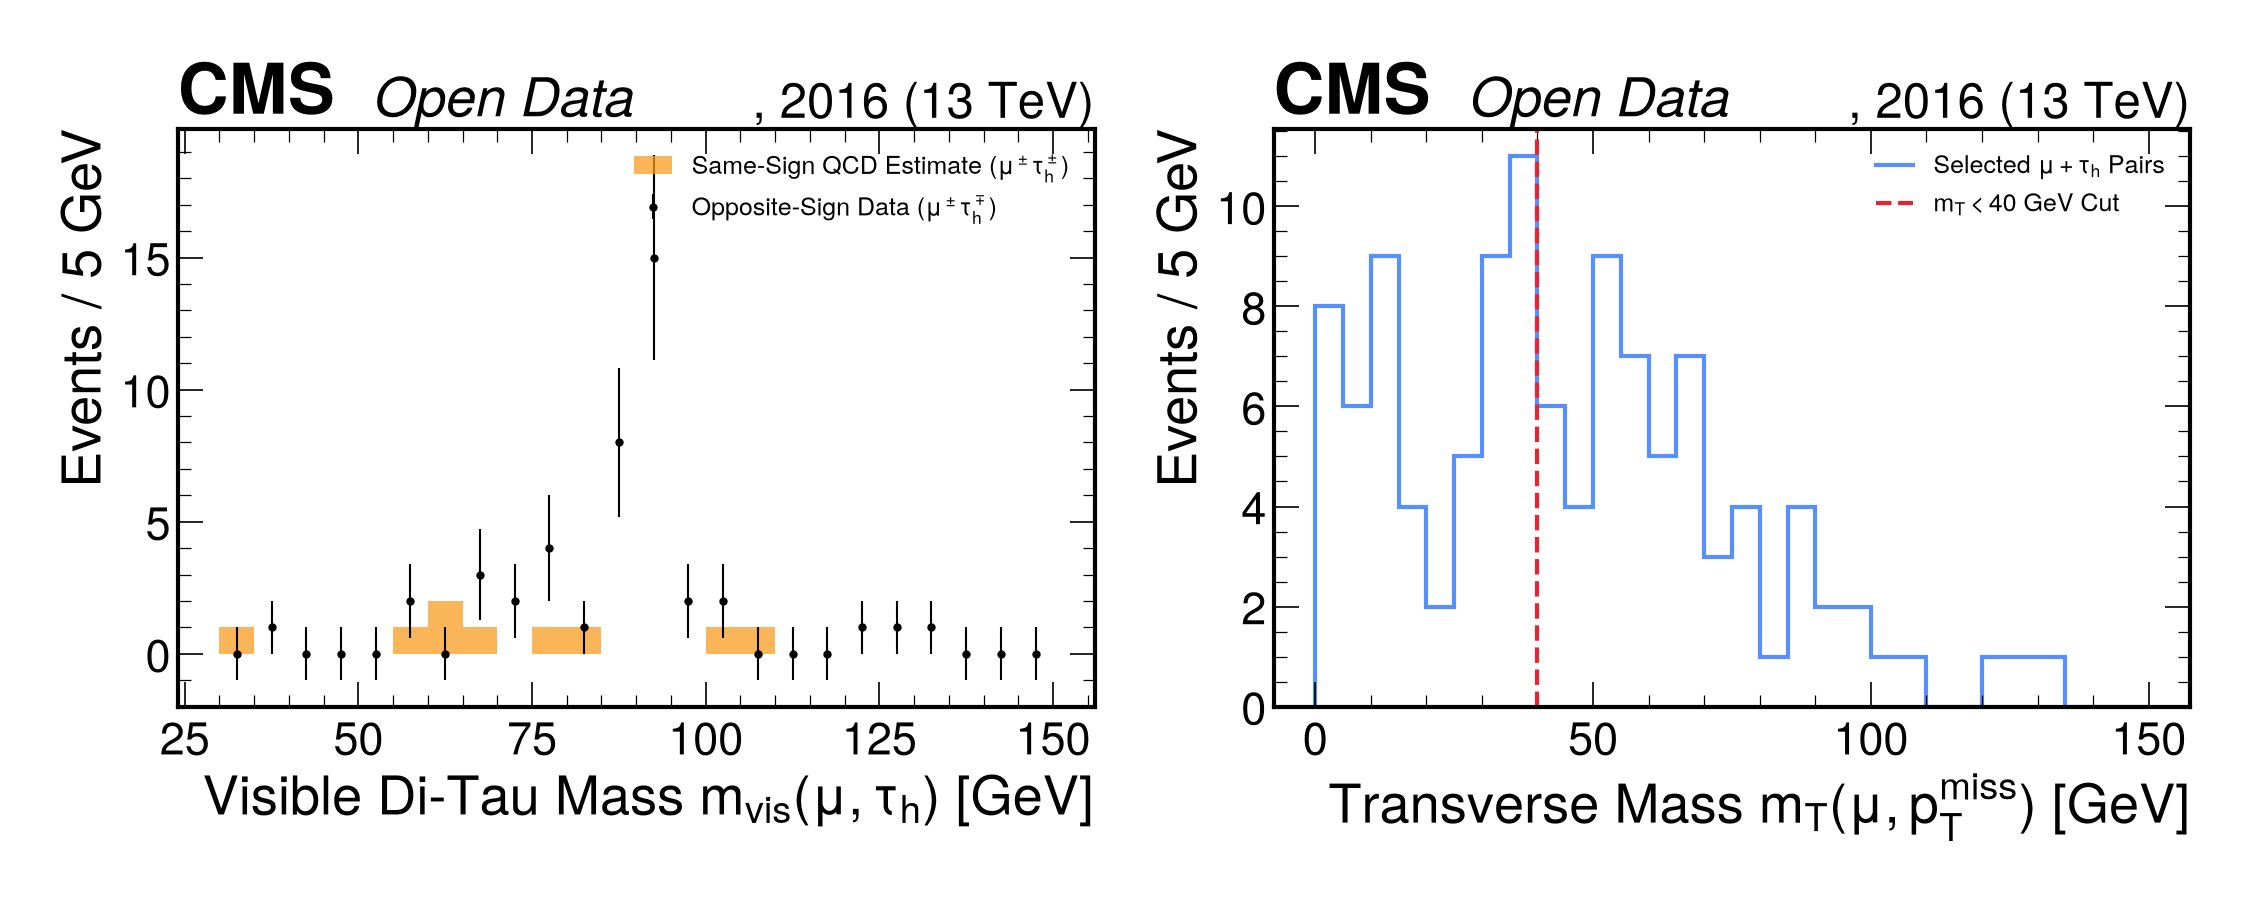
\includegraphics[width=0.98\textwidth]{../plots/cms_ditau_reconstruction.png}
    \caption{Left: Visible invariant mass $m_{\text{vis}}(\mu, \tau_h)$ in the low-$m_T$ signal region comparing Opposite-Sign data (black points) against the data-driven Same-Sign QCD background estimate (orange fill). Right: Transverse mass $m_T(\mu, p_T^{\text{miss}})$ distribution prior to the $m_T < 40\text{ GeV}$ cut (dashed red line).}
    \label{fig:recon}
\end{figure}

\section{Statistical Modeling with \texttt{RooFit}}
To quantify the resonant yield in the opposite-sign $m_{\text{vis}}(\mu, \tau_h)$ spectrum across $[30, 150]\text{ GeV}$, a composite probability density function is constructed in \texttt{RooFit}:
\begin{equation}
    \mathcal{P}(m_{\text{vis}}) = N_{\text{sig}} \cdot \mathcal{G}(m_{\text{vis}}; \mu, \sigma) + N_{\text{bkg}} \cdot \mathcal{E}(m_{\text{vis}}; \lambda),
\end{equation}
where $\mathcal{G}(m_{\text{vis}}; \mu, \sigma)$ denotes a Gaussian resonance model and $\mathcal{E}(m_{\text{vis}}; \lambda)$ represents an exponential continuum background. Figure~\ref{fig:roofit} and Table~\ref{tab:fit} present the maximum-likelihood fit results.

\begin{figure}[h!]
    \centering
    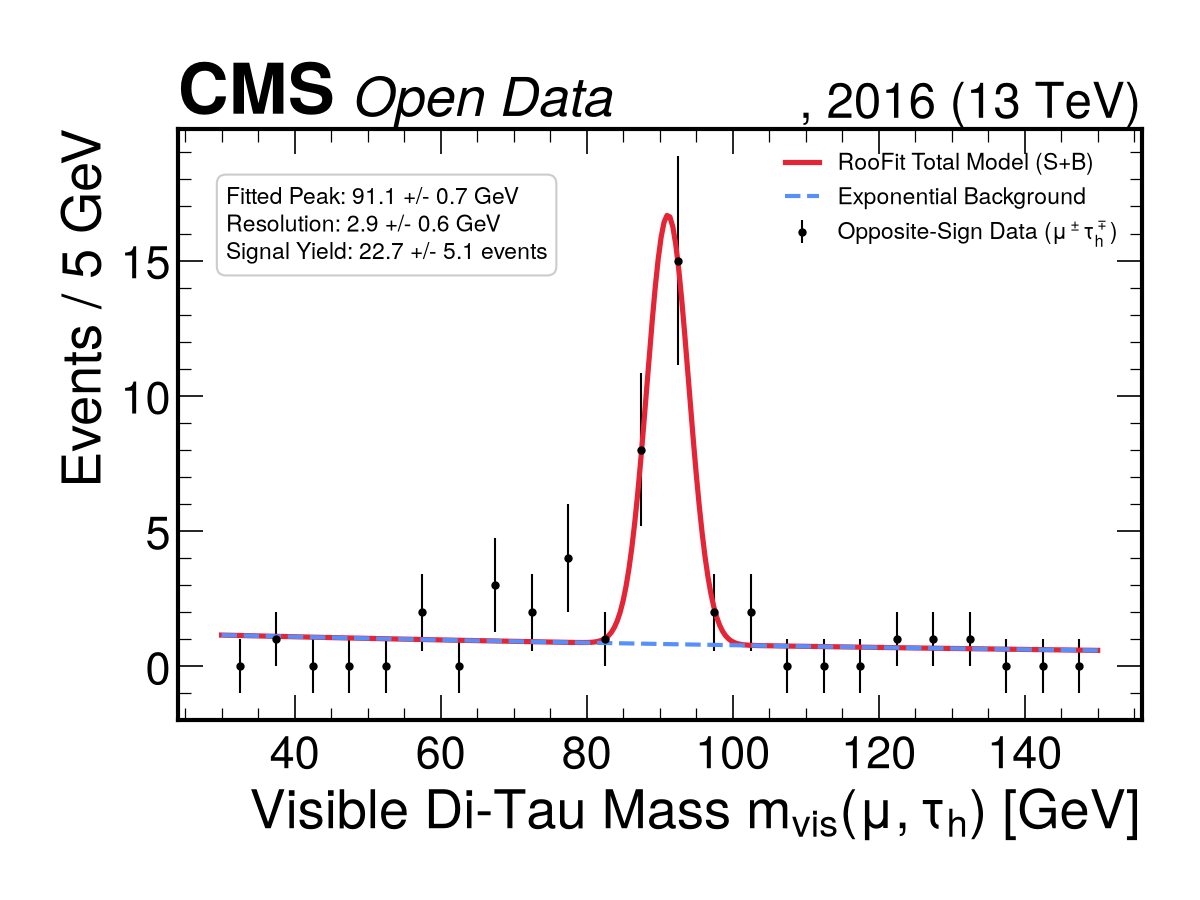
\includegraphics[width=0.68\textwidth]{../plots/roofit_mvis_fit.png}
    \caption{Maximum-likelihood fit to the Opposite-Sign $m_{\text{vis}}(\mu, \tau_h)$ distribution performed with \texttt{RooFit}, showing the total signal-plus-background model (solid red) and exponential continuum component (dashed blue).}
    \label{fig:roofit}
\end{figure}

\begin{table}[h!]
\centering
\caption{Extracted parameters from the \texttt{RooFit} maximum-likelihood fit.}
\label{tab:fit}
\begin{tabular}{lc}
\toprule
\textbf{Model Parameter} & \textbf{Fitted Value} \\
\midrule
Resonance Peak Mean ($\mu$) & $91.1 \pm 0.7\text{ GeV}$ \\
Detector Mass Resolution ($\sigma$) & $2.9 \pm 0.6\text{ GeV}$ \\
Extracted Signal Yield ($N_{\text{sig}}$) & $22.7 \pm 5.1\text{ events}$ \\
\bottomrule
\end{tabular}
\end{table}

The fitted peak position of $91.1 \pm 0.7\text{ GeV}$ is consistent with the nominal $Z$ boson mass ($91.19\text{ GeV}$), reflecting $Z \to \ell^+\ell^-$ events passing the baseline $\tau_h$ selection alongside the $60\text{--}80\text{ GeV}$ excess from $Z \to \tau^+\tau^-$. All C++ kinematic kernels are validated via automated \texttt{pytest} unit tests (\texttt{tests/test\_ditau\_kinematics.py}), and the full workflow is automated using \texttt{Snakemake} and \texttt{Docker}.

\begin{thebibliography}{9}
\bibitem{cms_nanoaod} CMS Collaboration (2024), \emph{SingleMuon primary dataset in NANOAOD format from RunH of 2016}, CERN Open Data Portal, DOI: \texttt{10.7483/OPENDATA.CMS.A342.9982}.
\bibitem{cms_workshop} CMS Open Data Group, \emph{Physics Analysis with CMS NanoAOD and RDataFrame ($H/\text{Z} \to \tau^+\tau^-$)}, CERN Open Data Workshop Documentation.
\end{thebibliography}

\end{document}
